\documentclass[fontset=ubuntu]{ctexart}

% \usepackage{ctex}
\usepackage{graphicx} % 图片
\usepackage{subfigure} %子图片
\usepackage{minted} % 代码
\usepackage{listings} % 代码
\usepackage{enumerate} % 有序列表
\usepackage{float} % 设置位置
\usepackage{hyperref} % 网页链接
\usepackage{fancyhdr} % 页眉页脚

\title{\Huge \textbf{实验报告一\\ Latex{} \& Git}}
\author{\textit{潘奕霖}}
\date{https://github.com/PLY1024/system-develop-tools\\ \today}
\pagestyle{fancy}

\fancyhead{}
\fancyhead[R]{\textsl{\leftmark}}
\fancyfoot{}
\fancyfoot[L]{https://github.com/PLY1024/system-develop-tools}
\fancyfoot[R]{\thepage}
\setlength{\headheight}{14pt}
\addtolength{\topmargin}{-5pt}

\begin{document}

\maketitle
\newpage

\tableofcontents
\newpage

\section{ \LaTeX 学习感悟}
\LaTeX 相比 Markdown 更具有上手难度,从一开始就需要记住代码,而且写错了就直接报错,比较有挫败感。不过比较让人欣慰的是在记住基本代码和折腾好格式之后, \LaTeX 基本上不需要在排版上耗费精力,不用像Word那样和无形的大手对抗,除了不能实时预览外,基本没什么缺点。而且格式模板的使用十分简单,有模板基本能做到Word那样的快速编辑。

在学习中遇到的最大的坑是Overleaf作为在线编译器,为编译中文而修改编译方式需要自行寻找一番,而且使用 \url{https://oi-wiki.org/tools/latex} 中的导入包方式会直接报错,
\begin{figure}[hbt]
    \centering
    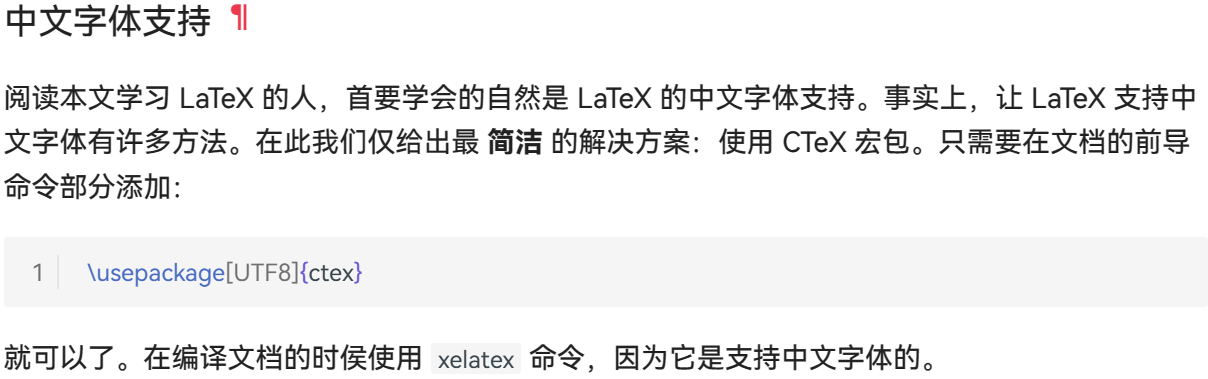
\includegraphics[width=0.5\linewidth]{chinese_1.png}
    \caption{ \LaTeX 文档中使用中文的方法}
    \label{fig:chinese_1}
\end{figure}
看起来Overleaf和utf-8有点矛盾。
\begin{figure}[hbt]
    \centering
    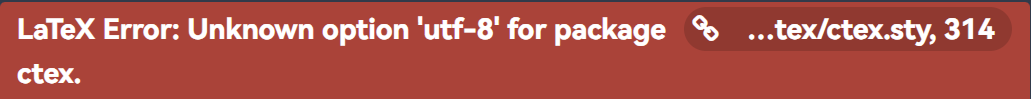
\includegraphics[width=0.5\linewidth]{error_1.png}
    \caption{Overleaf的报错信息}
    \label{fig:error_1}
\end{figure}

解决方法就是删掉[utf-8],或者文档类型使用ctexart。

Overleaf上比较折腾的是换字体。我个人不太喜欢默认的等宽字体,所以想着换成别的字体,但是上传字体之后总是一堆警告\textsuperscript{\ref{fig:warning_1}},让人很不爽,于是作罢。

\LaTeX 的自定义功能还是比较强大的,通过引入fancyhdr包能够自定义页眉和页脚。不过要注意在自定义的命令之前要先有\mintinline{Latex}|\fancyhead{}|这样的空命令以清空原有的设置,否则会发生冲突。通过指定R、C与L可以自定义页眉页脚不同位置的信息。我让右上角显示章名,左下角显示笔记仓库,右下角显示页码。值得一提的是显示章名的命令为\mintinline{Latex}|\leftmark|,而显示节名的命令为\mintinline{Latex}|\rightmark|,不要用错了。
\begin{figure}[htb]
    \centering
    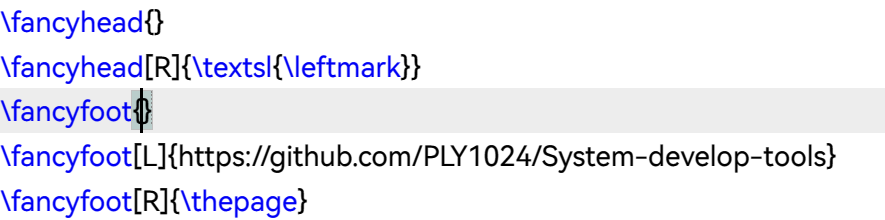
\includegraphics[width=0.75\linewidth]{custom_1.png}
    \caption{自定义页眉页脚}
    \label{fig:custom_1}
\end{figure}

以下是我所使用的包:
\begin{figure}[htb]
    \centering
    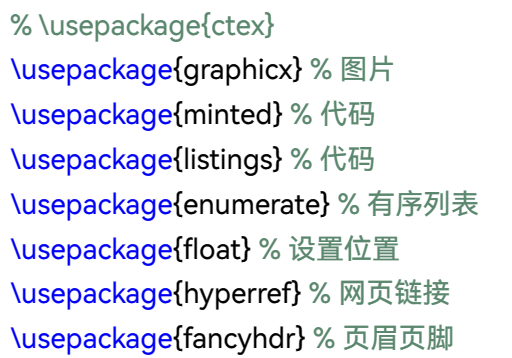
\includegraphics[width=0.5\linewidth]{package_1.png}
    \caption{使用的包}
    \label{fig:package_1}
\end{figure}

\section{ \LaTeX 知识点}
\subsection{ \LaTeX 安装}
可以在\url{https://www.tug.org/texlive/}下载TeX Live。 \LaTeX 有众多的编译器可以使用,我选择Overleaf作为编辑器,主要是其基于云端,基本开箱即用,并且能够实时编译,极大地省去了安装本地编译器的折腾过程。而且Overleaf可以辅助插入图片和列表,极大地省去了写命令的过程。

\subsection{源文件的基本结构}
分为导言区和正文区。导言区设定文档的格式,语言,导入需要的包。正文区用于显示文字、图表、公式等内容。

\subsection{内置文档格式}
 \LaTeX{} 内置了许多文档格式:
 \begin{itemize}
     \item article 文档
     \item report 报告
     \item book 书籍
     \item beamer 幻灯片
 \end{itemize}

\subsection{设置中文}
这是中文使用者使用 \LaTeX 遇到的最大困难之一,需要一定的操作,且网上的操作大多针对本地编译器,不一定对Overleaf生效。

在Overleaf中,点击左上角菜单,编译器选择为XeLatex,这是最为重要的一步,再导入ctex宏包,即可对中文进行编译。

若不导入ctex宏包,将文档类型设置为ctexart、ctexrep、ctexbook等格式也可以对中文进行编译。

注意,编译中文最重要的一步是修改编译器。还要注意的是两种方法会对文档的显示效果产生影响,ctexart的页眉会显示节名与页码,而普通article的页眉不会显示信息且页码位于页面底部。本报告使用的是ctexart类型的文档。

\subsection{消除“does not contain requested Script “CJK”.”警告}
Overleaf编译中文时会有非常经典的“CJK”警告,原因是Fandol字体没有GSUB表。通过在设置文档类型时指定编译平台的字符集,\LaTeX 就能使用平台自带的字体,避免Fandol字体的警告。Overleaf运行于Ubuntu,所以指定[fontset=ubuntu]。

\subsection{设置纸张大小和主要字号}
\mintinline{Latex}|\documentclass[a4paper, 10pt]{article}|将纸张大小设置为a4,主要字号大小设置为10pt。

\subsection{设置标题,作者,日期与目录}
设置标题:\mintinline{Latex}|\title{}|

设置作者:\mintinline{Latex}|\author|

设定日期为今日:\mintinline{Latex}|\date{\today}|

最后需要\mintinline{Latex}|\maketitle|以使标题生效,且以上的字体均可以改变字形和大小。在\mintinline{Latex}|\maketitle|后加上\mintinline{Latex}|\newpage|可以让标题单独成页。

在使用\mintinline{Latex}|\tableofcontents|后 \LaTeX 会自动生成目录,同样可以单独成页。

\subsection{设置章、节、小节}
\begin{itemize}
    \item \mintinline{Latex}|\section{}| 设置节
    \item \mintinline{Latex}|\subsection{}| 设置小节
    \item \mintinline{Latex}|\subsubsection{}| 设置小小节
    \item \mintinline{Latex}|\chapter{}| 设置章
    \item \mintinline{Latex}|\part{}| 设置部
\end{itemize}

注意,chapter与part需要在book类型的文档中使用。

\subsection{设置换行}
偶然发现\mintinline{Latex}|\\|可以将文本换行,就像\\这样。

\subsection{设置分段}
在文段间空一行可以实现对文字的分段,在文段中回车并不能将文段分段。

\subsection{自定义字体}
将字体文件上传至.tex文件所在文件夹,在文档开头添加以下命令:
\mintinline{Latex}|\setmonofont{MapleMono.ttf}|就可以自定义等宽字体。但是MapleMono字体在报告中显示效果不佳,本报告就使用默认的等宽字体。
同样的,将字体文件上传后在文档开头添加\mintinline{Latex}|\setCJKmainfont{}|也可以修改默认字体,但是造成一堆warning。
\begin{figure}[htb]
    \centering
    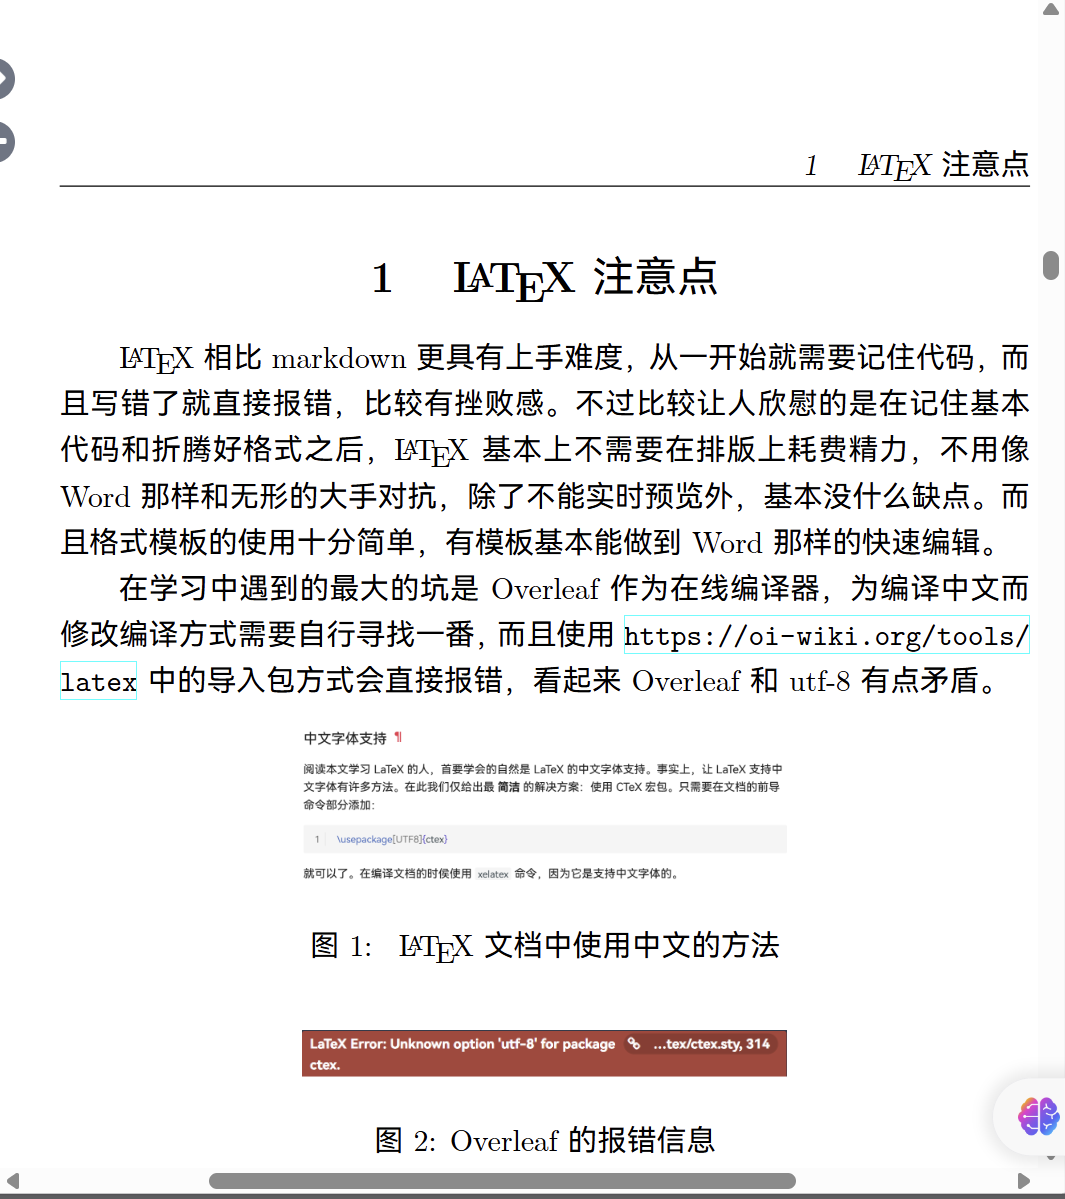
\includegraphics[width=0.5\linewidth]{font_1.png}
    \caption{更换字体的效果}
    \label{fig:font_1}
\end{figure}

\begin{figure}[htb]
    \centering
    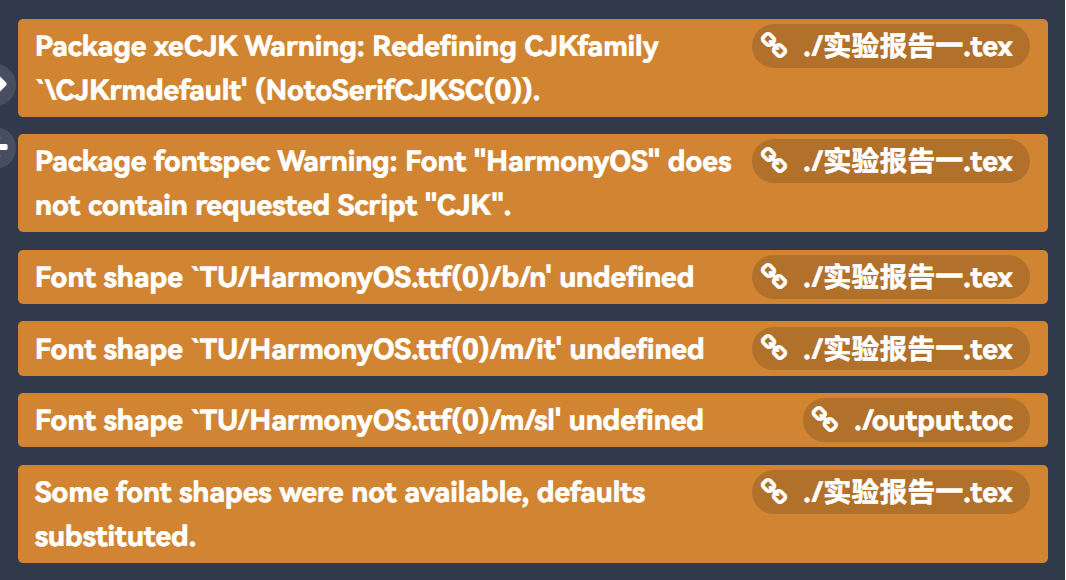
\includegraphics[width=0.5\linewidth]{warning_1.png}
    \caption{一堆警告}
    \label{fig:warning_1}
\end{figure}

\subsection{字体类型设置}
若不使用自己添加的字体,可以通过改变字形以在 \LaTeX 中显示不同的字体。

\subsubsection{粗体}
\mintinline{Latex}|\textbf{}|,\textbf{这是粗体}, \textbf{word}.

\subsubsection{斜体}
\mintinline{Latex}|\textit{}|,\textit{这是斜体},\textit{word}.

\subsubsection{无衬线字体}
\mintinline{Latex}|\textsf{}|,\textsf{这是无衬线字体},\textsf{word}.

\subsubsection{等宽字体}
\mintinline{Latex}|\texttt{}|,\texttt{这是等宽字体},\texttt{word}.

\subsubsection{罗马字体}
\mintinline{Latex}|\textrm{}|,\textrm{这是罗马字体},\textrm{word}.

可以看到,所谓罗马字体就是默认字体。

\subsubsection{使用下划线}
\mintinline{Latex}|\underline{}|,\underline{这是下划线},在这里非常不恰当地将下划线分类到字形类型设置中。

\subsection{字号设置}
通过\mintinline{Latex}|\large|等命令来设置字体的大小,这就是{\large 随意}{\small 设置}{\tiny 的}{\Huge 效果}。

\subsection{显示 \LaTeX Logo}
使用\mintinline{Latex}| \LaTeX |命令显示 \LaTeX Logo,类似的,还可以显示 \LaTeXe , \TeX 等Logo。

注意,命令的前后一定要各留有一个空格,否则会有奇怪的报错产生。

\subsection{使用代码}
\mintinline{Latex}|\begin{verbatim} \end{verbatim}|与\mintinline{Latex}|\verb|||命令能够将其内容以纯文本形式显示,因此可以用于显示代码。

通过引入minted和listings包,也能实现显示代码的效果,不同的是minted包通过在指定编程语言后能够支持代码高亮,因而显示效果更佳。

\subsubsection{行内代码}
\begin{itemize}
    \item \mintinline{Latex}|\verb|||:\verb|print("Man!")|
    \item \mintinline{Latex}|\mintinline{Python}|||:\mintinline{Python}|print("Man!")|
\end{itemize}

\subsubsection{代码块}
通过\mintinline{Latex}|\begin{verbatim} \end{verbatim}|显示纯文本的代码块:
\begin{verbatim}
    import time
    print("Man!")
\end{verbatim}


通过以下代码显示带高亮的代码块:
\begin{verbatim}
    \begin{listing}[htb]
        \begin{minted}{Python}

        \end{minted}
    \end{listing}
\end{verbatim}

\begin{listing}[htb]
	\begin{minted}{Python}
    import time
    print("Man!")
    \end{minted}
\end{listing}

\mintinline{Latex}|\mint{}|||还能显示单独成行的代码。

\subsection{列表}
\subsubsection{无序列表}
使用\mintinline{Latex}|\begin{itemize} \end{itemize}|设定列表环境,在
\mintinline{Latex}|\item|后接列表内容,还可以自定义行标。 
\begin{itemize}
    \item 列表内容1
    \item[*] 列表内容2
\end{itemize}

\subsubsection{有序列表}
使用\mintinline{Latex}|\begin{enumerate} \end{enumerate}|设定有序列表,同样可以自定义行标,不过需要引入enumerate包。
\begin{enumerate}[1)]
    \item 列表内容1
    \item 列表内容2
\end{enumerate}

\subsection{显示图片}
需要引入graphicx包,用\mintinline{Latex}|\begin{figure} \end{figure}|设定图片环境,通过\mintinline{Latex}|\includegraphics[width=0.5\textwidth]{path}|显示图片并设置图片大小。可以用\mintinline{Latex}|\centering|设置图片居中,
\mintinline{Latex}|\caption{title}|设置图片标题,注意图片的标题需要位于图片的下方。

\begin{figure}[htb]
\centering

\includegraphics[width=0.75\textwidth]{big_sur_1.jpg}
\caption{标题需要位于图片的下方}
\end{figure}

\subsection{显示公式}
显示行内公式:\mintinline{Latex}|$equation$|,如质能方程$E = mc^2$。

\mintinline{Latex}|\begin{equation} \end{equation}|设定公式环境
或简写为\mintinline{Latex}|\[ \]|。
\[
E = mc^2
\]
复杂公式
\[
d = {k \varphi(n) + 1} \over e
\]
\mintinline{Latex}|\frac{}{}|也可以显示分数。

可以借助在线公式网站\url{https://editor.codecogs.com/}辅助公式的编辑.

\subsection{显示表格}
\mintinline{Latex}|\begin{table}[h] \end{table}|设定表格环境,\mintinline{Latex}|\caption{title}|设置表格标题,在\mintinline{Latex}|\begin{tabular}{c c c} \end{tabular}|之间设置表格内容。表格格式中c代表格内内容居中,l、r代表左、右对齐,p可以自由设定宽度,自动换行,c、l、r间可以添加分割标记,|与||形成不同的分隔。\mintinline{Latex}|\hline|添加横向分割,用法类似|。表格的内容通过\&分隔,以双斜杠进行换行。\mintinline{Latex}|\centering|可以居中显示表格。可以对表格进行引用。注意,表格的标题要放置于表格上方。
\begin{table}[htb]
    \centering
    \caption{标题要放置于表格上方}
    \begin{tabular}{c||c}
        \hline\hline
        内容1 & 内容2 \\
        \hline
        内容3 & 内容4 
    \end{tabular}
    \label{tab:my_label}
\end{table}

\subsection{设置引用}
用\mintinline{Latex}|\label{label}|设置引用时的标签,用\mintinline{Latex}|\ref{label}|进行引用。

这是一段话\label{1}。

这是对一段话的引用\ref{1}。

对于有标题的环境类型来说,标签需要设定于标题后。

\subsection{显示超链接}
导入hyperref包:\mintinline{Latex}|\usepackage{hyperref}|,使用\mintinline{Latex}|url{}|命令显示超链接。

笔记仓库:\url{https://github.com/PLY1024/system-develop-tools}

\subsection{设置浮动位置}
在浮动体开始代码处的\mintinline{Latex}|[]|内可以放置!htbp等字符,用于设置浮动块的位置。

\begin{itemize}
    \item h 放置此处
    \item t 放置本页顶部
    \item b 放置本页底部
    \item p 放置于某一专门页面
\end{itemize}

四个字母可以连用,一般使用htb,!代表覆盖 \LaTeX{} 的放置策略,H代表将内容准确地放置于代码所在的位置,需要引入float包,不过一般不使用。

\section{Git学习感悟}
Git的概念比较抽象,最开始不太好理解,并且同样是一开始便需要记住命令。个人觉得比较好的方法是找一个视频跟着敲一敲代码,熟悉一下流程。比较麻烦的是Github的注册和使用,需要特殊手段,使用Gitee虽然是一种解决方案,但感觉上始终不太对。

以下是个人总结的Git使用流程:先获取一个仓库,无论是初始化本地文件夹为仓库还是克隆远程仓库;再对本地文件进行跟踪,进行一次提交,这样就对本地文件进行了一次快照;接着就可以对文件进行修改,在修改后暂存文件并进行提交。还可以连接远程仓库,将本地的修改推送到远程仓库。

\section{Git知识点}
\subsection{安装}
\subsubsection{Linux}
对于基于Debian的发行版,使用如下命令安装:\mint{shell}|sudo apt install git-all|

我的WSL安装的是Arch Linux,使用如下命令安装:\mint{shell}|pacman -S git|

\subsubsection{Windows}
Windows可以访问\url{https://git-scm.com/download/win}下载 Git for Windows 项目,或访问\url{https://git-scm.com/downloads/guis}下载Git GUI 客户端。

\subsection{初始配置}
\subsubsection{配置基本信息}
设置用户名和邮箱,其中\mintinline{shell}|--globe|选项使得这样的配置成为全局配置,为以后的项目所使用。
\mint{shell}|git config --global user.name "<username>"|
\mint{shell}|git config --global user.email <mailbox>|

\subsubsection{设置文本编辑器}
文本编辑器在Git需要你输入信息时调用,在未配置时使用的是操作系统的默认文本编辑器。通过以下命令设置vim为文本编辑器。
\mint{shell}|git config --global core.editor <editor name>|

\subsection{查看配置}
查看所有Git能找到的配置:
\mint{shell}|git config --list|
通过在末尾添加\mintinline{shell}|--show-origin|显示配置所在的文件。

\subsection{获得帮助}
通过如下三种方法获取Git的命令手册:
\mint{shell}|git help <verb>|
\mint{shell}|git <verb> help|
\mint{shell}|man git-<verb>|
或通过在命令末尾添加\mintinline{shell}|-h|来获得某个命令的简明帮助。

\subsection{日志操作}
通过以下命令查看提交日志:\mintinline{shell}|git log|,日志中HEAD所指向的是当前分支。
\begin{figure}[htb]
    \centering
    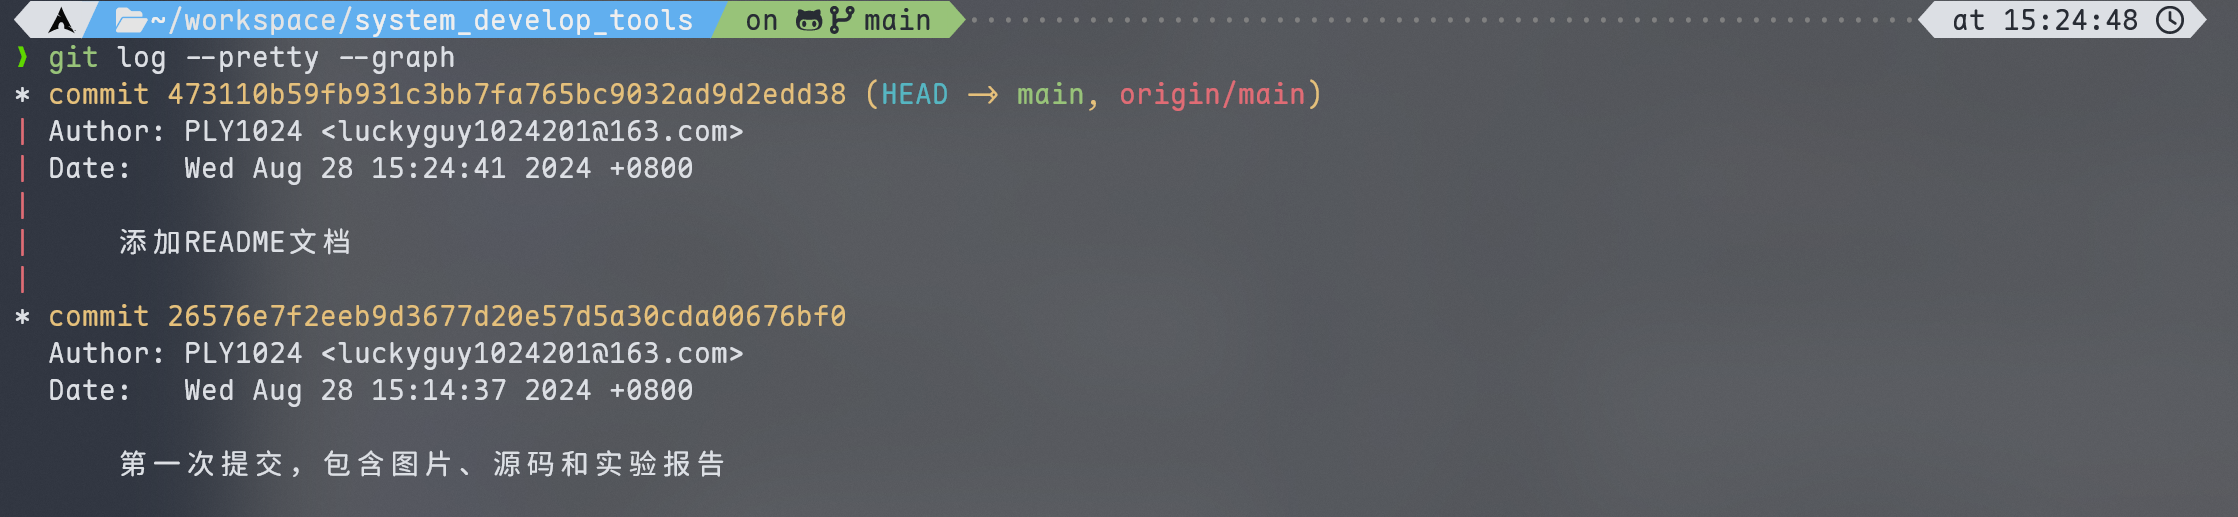
\includegraphics[width=0.75\linewidth]{git_log_1.png}
    \caption{Git log}
    \label{fig:git_log_1}
\end{figure}

一些常用选项:
\begin{itemize}
    \item \mintinline{shell}|--all| 显示所有分支上的提交,包括远程仓库
    \item \mintinline{shell}|--patch| 显示每次提交所引入的差异
    \item \mintinline{shell}|--stat| 显示简略统计信息
    \item \mintinline{shell}|--pretty| 设置输出格式
    \item \mintinline{shell}|-n| 显示最近n次提交
\end{itemize}

\subsubsection{输出格式选项\mintinline{shell}|--pretty|}
将每个提交信息在一行内显示:\mintinline{shell}|git log --pretty=oneline|

自定义输出格式:\mintinline{shell}|git log --pretty=format:"%h %an %ad: %s"|
\begin{itemize}
    \item \%H 显示提交的完整哈希
    \item \%h 显示提交的简写哈希
    \item  \%an 显示作者名字
    \item  \%ad 显示修改日期 
    \item  \%ar 显示距今修改日期 
    \item  \%s 显示提交说明 
\end{itemize}

形象地显示分支变化:\mintinline{shell}|git log --graph|,可以与\mintinline{shell}|--pretty|连用。

\subsection{获取Git仓库}
\subsubsection{在本地目录初始化仓库}
在需要初始化的文件夹下执行:\mintinline{shell}|git init|,将该文件夹初始化为Git仓库。执行以下命令来追踪指定的文件并进行初始提交。
\mint{shell}|git add <filename>|
\mint{shell}|git commit -m '<message>'|
\begin{figure}[htb]
    \centering
    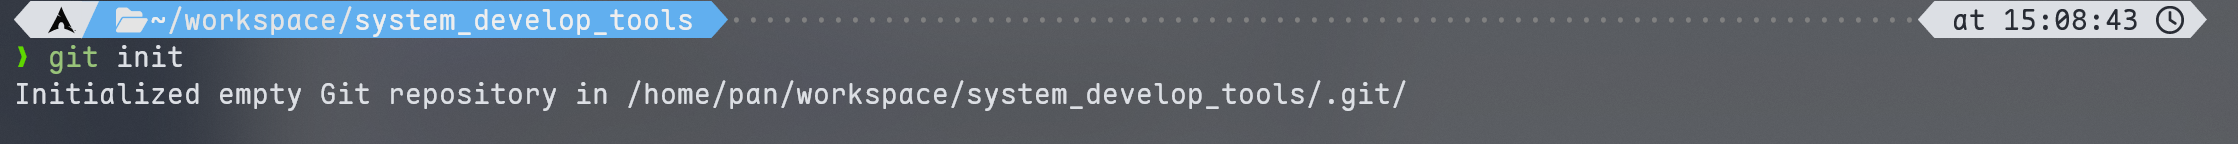
\includegraphics[width=0.75\linewidth]{git_init_1.png}
    \caption{Git init}
    \label{fig:git_init_1}
\end{figure}

\subsubsection{克隆远程仓库}
通过执行\mintinline{shell}|git clone <url>|,将在当前目录下创建一个与所克隆仓库同名的文件夹,其中包含仓库中的所有项目文件,也可以添加\mintinline{shell}|<dirname>|来自行指定本地文件夹名称。

Git支持https://或SSH协议与远程仓库进行连接。

\subsection{查看当前文件状态}
使用\mintinline{shell}|git status|查看仓库内文件所处的状态,添加\mintinline{shell}|-s|选项使得输出更加简洁。对于一个提交后未更改文件的仓库来说,当前的工作目录是“clean”的。\mintinline{shell}|git status|命令会列出当前所在的分支,未跟踪的文件(即未被提交过的文件),与暂存中的文件(即在执行提交命令时会被提交的文件)。通过执行\mintinline{shell}|git add|对文件进行跟踪,意味着将该文件添加到下次提交的内容中。
\begin{figure}[htb]
    \centering
    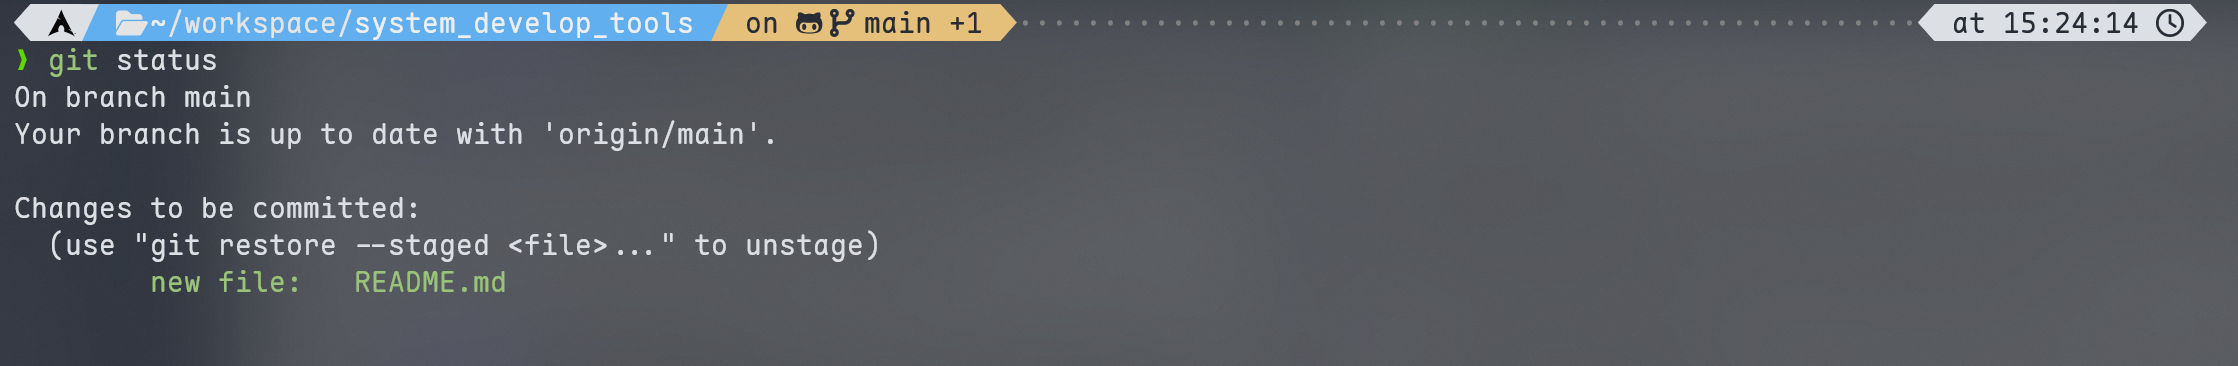
\includegraphics[width=0.75\linewidth]{git_status_1.png}
    \caption{Git status}
    \label{fig:git_status_1}
\end{figure}

注意,\mintinline{shell}|git commit -m '<message>'|命令提交的是暂存区中的文件,而非工作目录内的文件。

创建.gitignore文件可以配置需要忽略提交的文件格式。

\mintinline{shell}|git diff|命令可以查看工作目录中当前文件与暂存区文件的差异,即尚未暂存的改动。

\subsection{提交更新}
提交命令\mintinline{shell}|git commit|会启动文本编辑器,添加\mintinline{shell}|-m '<message>'|可以直接输入提交说明。
\begin{figure}[htb]
    \centering
    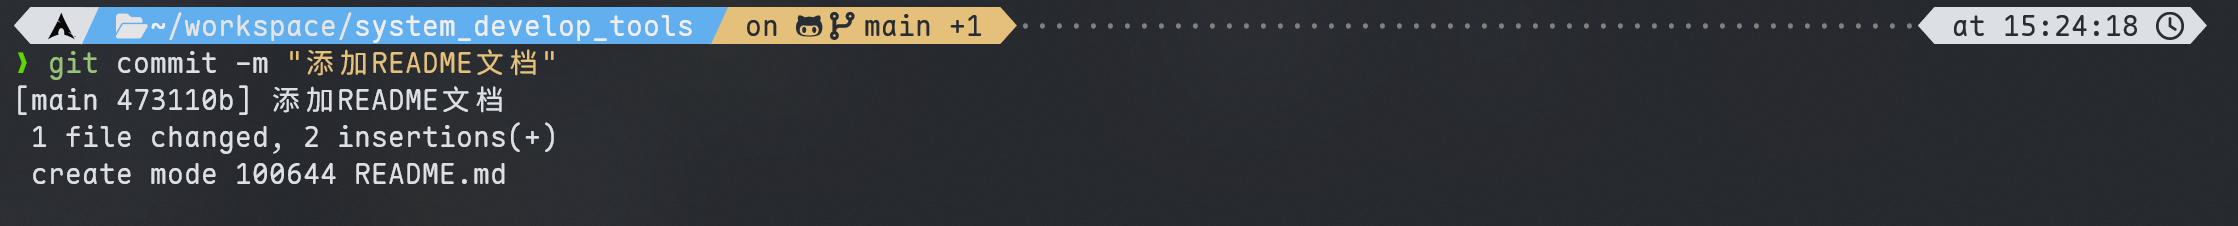
\includegraphics[width=0.75\linewidth]{git_commit_1.png}
    \caption{Git commit}
    \label{fig:git_commit_1}
\end{figure}

通过添加\mintinline{shell}|-a|选项使Git自动将已跟踪文件暂存并提交,略过\mintinline{shell}|git add|步骤。

注意,提交时记录的是暂存区的文件,未暂存的文件不会被提交。

\subsection{移除文件}
\subsubsection{仅从暂存区移除文件}
\mint{shell}|git rm --cached <filename>|

\subsubsection{从暂存区移除文件并删除}
\mint{shell}|git rm <filename>|

\subsection{链接远程仓库}
在Github构建一个远程仓库,通过\mintinline{shell}|git remote add <name> <url>|链接该仓库,可以自己设定该仓库在本地显示的名称。执行\mintinline{shell}|git remote|显示远程仓库名,使用\mintinline{shell}|git remote rename <oldname> <newname>|可以修改本地显示的仓库名。

\subsection{移除远程仓库}
\mintinline{shell}|git remote remove|以移除远程仓库。

\subsection{从远程仓库拉取或抓取}
\subsubsection{fetch}
\mintinline{shell}|git fetch <remote>|会拉取远程仓库中本地所没有的数据,在执行完成后会显示远程仓库中所有分支的引用,需要对分支进行手动合并。

\subsubsection{clone}
\mintinline{shell}|git clone <url>|克隆远程仓库,并默认命名为origin。

\subsubsection{pull}
\mintinline{shell}|git pull <remote>|以抓取数据并自动尝试合并到当前分支。

\subsection{推送本地分支}
\mintinline{shell}|git push origin main|以将本地的main分支推送到origin仓库。\mintinline{shell}|-u|使得将来使用\mintinline{shell}|git push|即可向仓库推送更改。
\begin{figure}[htb]
    \centering
    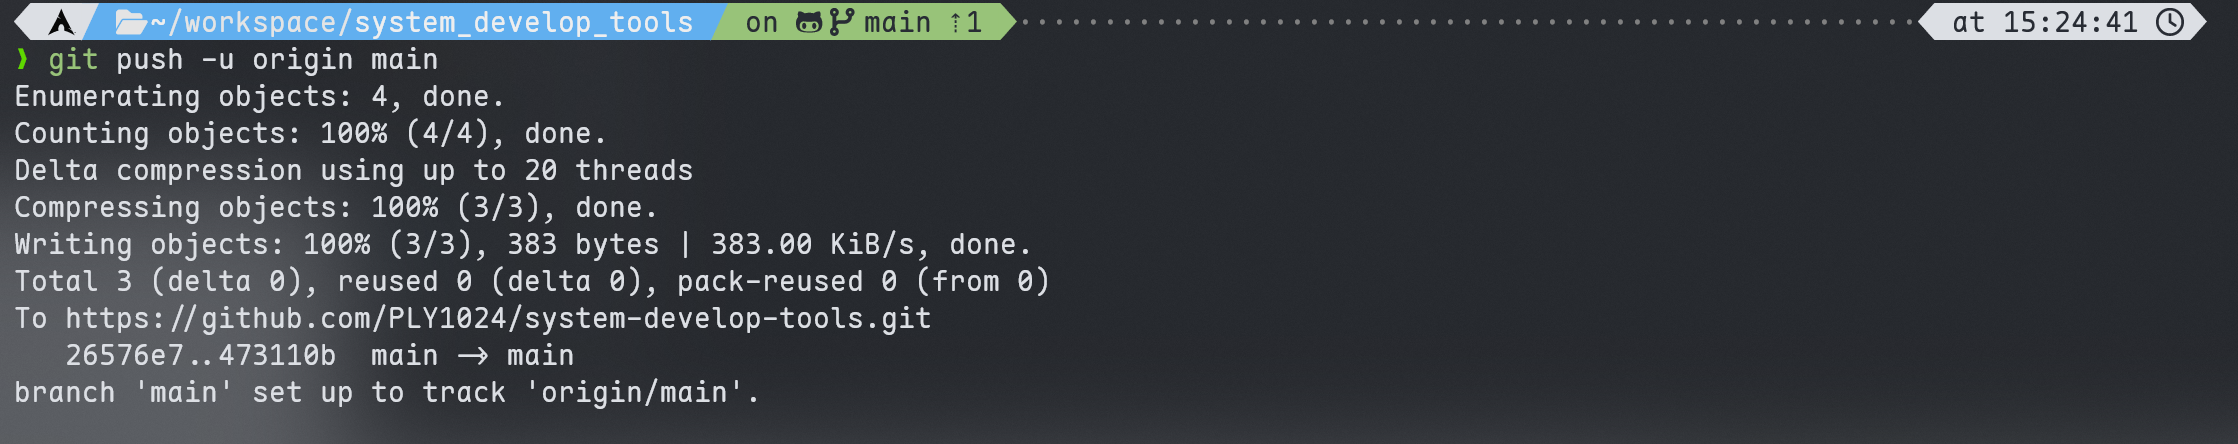
\includegraphics[width=0.75\linewidth]{git_push_1.png}
    \caption{Git push}
    \label{fig:git_push_1}
\end{figure}

\subsubsection{使用token推送项目}
在Github的个人主页下,Settings->Developer settings->Personal access tokens获取一个token,在\mintinline{shell}|git push|命令要求输入密码时使用。

注意,\mintinline{shell}|git config --global credential.helper store|命令可以保存账号名和token,下次推送时无需再次输入。

\subsubsection{使用SSH密钥推送项目}
在shell运行\mintinline{shell}|ssh-keygen -t rsa -C “<mailbox>”|生成SSH密钥,在Github添加公钥进行配对。通过运行
\mintinline{shell}|ssh -T git@github.com|以验证是否成功。

\subsection{撤销提交}
\mintinline{shell}|git reset HEAD~ --soft|,在\mintinline{shell}|~|后跟数字指定撤销过去某一次的提交。
不同参数的意义:
\begin{itemize}
    \item \mintinline{shell}|--soft|代表撤销提交但仍在暂存区中保留文件
    \item \mintinline{shell}|--hard|代表撤销提交且复原回上一次提交时的状态,所有的修改都会丢失
    \item 不加参数代表撤销提交,且不在暂存区中保留文件,但所做的修改仍然存在
\end{itemize}

\subsection{分支操作}
\subsubsection{查看分支}
\mintinline{shell}|git branch --list|,其中\*所处的是当前分支.

\subsubsection{创建新分支}
\mintinline{shell}|git branch <branchname>|

\subsubsection{切换分支}
\mintinline{shell}|git checkout <branchname>|

\subsubsection{新建分支并直接切换}
\mintinline{shell}|git checkout -b <branchname>|

\subsubsection{合并分支}
\mintinline{shell}|git merge <branchname>|

\subsubsection{删除分支}
\mintinline{shell}|git branch -d <branchname>|

\subsection{将远程仓库中的分支变为本地分支}
主要在\mintinline{shell}|git fetch <remote>|后执行,有三种不同的命令,但效果相同:
\mint{shell}|git checkout  <branchname>|
\mint{shell}|git checkout -b <branchname> <remote path>|
\mint{shell}|git checkout  --track <remote path>|

\mintinline{shell}|<remote path>|指的是该远程分支在远程仓库中的路径。

\subsection{当前工作文件的储存与恢复}
\mintinline{shell}|git stash|命令可以保存当前工作目录下所有正在修改的文件。

\mintinline{shell}|git stash apply|可以重新加载这些文件。

\subsubsection{多次存储}
\mintinline{shell}|git stash push|将文件当前的修改存储为一个副本。

\mintinline{shell}|git stash list|能列出存储的文件列表,序号由小到大表示存储时间由近到远。

\subsubsection{恢复储存的文件}
\mintinline{shell}|git stash pop|将文件恢复为最近一次保存的状态,并删除该次备份。

\mintinline{shell}|git stash apply stash@{<number>}|则可以恢复某次储存的文件。

\subsubsection{删除某一次备份}
\mintinline{shell}|git stash drop stash@{<number>}|删除指定的备份文件。

\subsection{复原文件为仓库中保存的状态}
\mintinline{shell}|git checkout -- <filename>|,即使用库中的文件替换掉本地的文件。

\subsection{变基}
\mintinline{shell}|git rebase {branchname}|相当于在另一个分支上进行了本分支的修改,还可以指定对前n次提交进行修改:\mintinline{shell}|git rebase -i HEAD~{<number>}|

\end{document}